% -*- TeX:UTF-8 -*-

\documentclass[10pt,xcolor={svgnames},t]{beamer}
% 이곳에서는 글씨체의 크기를 10 pt로 하였음, t는 본문 내용이 슬라이드의 위(top)부터 시작

\mode<presentation> 									% 출력 양식을 프레젠테이션으로
{
	\usetheme{Boadilla}      							% 템플릿은 프랑크푸르트로

% 템플릿 종류: Antibes, Bergen, Berkerley, Berlin, Boadilla, Copenhagen, Darmstadt, Dresden, Frankfurt, Goettingen,
%  Hannover, Ilmenau, JuanLesPins, Luebeck, Madrid, Malmoe, Marburg, Montpellier, PaloAlto, Pittsburgh, Rochester,
%  Singapore, Szeged, Warsaw
%
%	\usecolortheme[named=orange]{structure}		% 색상 결정
 	\usefonttheme[onlymath]{serif}					% 수학공식에서 사용하는 글씨체
  % \useoutertheme{infolines}
  % or whatever

  %\setbeamercovered{transparent}						% overlay 사용
  % or whatever (possibly just delete it)
}
\setbeamerfont{block body}{size=\small}

%==================  필요한 패키지 설정 ===============
\usepackage{verbatim}
\usepackage{pdfpages}
\usepackage{multimedia}
\usepackage{animate}
\usepackage{wrapfig}
%
\usepackage{bm}% mathbf math
\usepackage{amsmath,amssymb,amscd}
\usepackage{subeqnarray}
\usepackage{mathptmx}
%
\usepackage{helvet}
\usepackage{courier}
\usepackage{relsize}
%
\usepackage{colortbl}
\usepackage{wasysym}
%

\usepackage{tikz}
\usetikzlibrary{arrows,shapes,calc,patterns}
\tikzstyle{every picture}+=[remember picture]
\usetikzlibrary{%
    decorations.pathreplacing,%
    decorations.pathmorphing%
}
% ================== 한글 사용 =====================
\usepackage{dhucs}
\usepackage{ifpdf}
\ifpdf
  \input glyphtounicode\pdfgentounicode=1
\fi
%==============================================
%
%================ dual screen =======================
%\setbeameroption{show notes on second screen=left}
%\setbeamertemplate{note page}[compress]
%==============================================
%
%================ 제목에 사용할 글씨체 설정 ==============
%\setbeamerfont{title}{shape=\itshape,family=\rmfamily}
%\setbeamerfont{frametitle}{family=\rmfamily}
%\usepackage[T1]{fontenc}
% Or whatever. Note that the encoding and the font should match. If T1
% does not look nice, try deleting the line with the fontenc.
%===============================================
%
%==================  표지 만들기 =====================
\title[Generalized Linear Models] % (optional, use only with long paper titles)
{Generalized Linear Models}
\subtitle{}


\author[Jin Hyun Nam]{Jin Hyun Nam }													% 저자(발표자)
\def\coauthors{JH Nam}
% Till Tantau\author{{1} \and
% J\"{o}rg Cassens\inst{2}

\institute[] 															% (optional, but mostly needed) 소속기관 약자 표기
{}													% 표지에 나타나는 소속기관 full name
% - Use the \inst command only if there are several affiliations.
% - Keep it simple, no one is interested in your street address.

\date[Aug 12, 2020]
 {Aug 12, 2020}														% (optional, should be abbreviation of conference name)
{}		
																	% 날짜 지정: \today
% - Either use conference name or its abbreviation.
% - Not really informative to the audience, more for people (including
%   yourself) who are reading the slides online

\subject{Beamer}
% This is only inserted into the PDF information catalog. Can be left out.

% Delete this, if you do not want the table of contents to pop up at
% the beginning of each subsection:
%===============================================
%
% ====================  차 례 ======================
 \AtBeginSection[]
 {
 \begin{frame}<beamer>
    \frametitle{Contents}
    \tableofcontents[currentsection,hideallsubsections]
    %\tableofcontents[currentsection,currentsubsections]
  \end{frame}
}
%===============================================
%
%
%==========================  본문 시작 ==============================
\begin{document}
%
%=================  표지를  화면으로 나타나기 =============
\begin{frame}
  \titlepage

\end{frame}
%===============================================
%
%=================  전체 목차 나타내기 =============
%\begin{frame}
 %   \frametitle{차 례}
  %  \tableofcontents[allsection,hidesubsections]
%\end{frame}
%===============================================

% ******************************
\section{Generalized Linear Models}
%*******************************
%
%
%------------------------------- 슬라이드   --------------------------------------------------
\begin{frame}
	\frametitle{The General Linear Model}
	
	\bigskip
	\begin{block}{The \textbf{general linear model}}
		\bigskip
		\begin{displaymath}
		y_i = \beta_0 + \beta_1 x_{1i} + \ldots + \beta_p x_{pi} + \epsilon_i
		\end{displaymath}
		\\
		the \textbf{response} $y_i$, $i=1,\ldots ,n$ is modelled by a linear function of \textbf{explanatory} variables $x_j$, $j=1 , \ldots , p$ plus an error term.
	\end{block}
	\bigskip
	
	
\end{frame}
%------------------------------------------------------------------------------------------
%
%------------------------------- 슬라이드   --------------------------------------------------
\begin{frame}
	\frametitle{General and Linear}
	
	\begin{itemize}
		\item Here general refers to the dependence on potentially more than one explanatory variable, v.s. the simple linear model:
		\[
		y_i = \beta_0 + \beta_1 x_i + \epsilon_i
		\]
		
		\item The model is linear in the parameters, e.g.
		\begin{eqnarray*}
			y_i &=& \beta_0 + \beta_1 x_1 + \beta_2 x_1^2 + \epsilon_i \\
			y_i&=&\beta_0 + \beta_1 x_1x_2 + \beta_2 exp(x_2) +\epsilon_i
		\end{eqnarray*}
		but not e.g.
		\begin{eqnarray*}
			y_i &=& \beta_0 + \beta_1 x_1^{ \beta_2}+ \epsilon_i \\
			y_i&=&\beta_0 exp(\beta_1 )x_1 +\epsilon_i
		\end{eqnarray*}
	\end{itemize}
	
	
\end{frame}
%------------------------------------------------------------------------------------------
%

%
%
%------------------------------- 슬라이드   --------------------------------------------------
\begin{frame}
	\frametitle{Error Structure}
	
	\begin{itemize}
		\item We assume that the errors $\epsilon_i$ are independent and identically distributed such that
		\[ E[\epsilon_i]=0 \hskip5pt
		\text{and} 
		\hskip5pt var[\epsilon_i]=\sigma^2
		\]
		\bigskip
		\item Typically we assume 
		\[
		\epsilon_i \sim N(0 , \sigma^2 )
		\]
		as a basis for inference, e.g. t-tests on paramters.
	\end{itemize}
	
	
\end{frame}
%------------------------------------------------------------------------------------------
%
%
%
%------------------------------- 슬라이드   --------------------------------------------------
\begin{frame}
	\frametitle{Restrictions of Linear Models}
	
	\begin{itemize}
		\item Although a very useful framework, there are some situations where general linear models are not appropriate.
		\begin{itemize}
			\item the range of $Y$ is restricted (e.g. binary, count)
			\item the variance of $Y$ depends on the mean
		\end{itemize}
		\bigskip
		\item Generalized linear models (GLMs) extend the range of application of general linear models by accommodating response variables with non-normal conditional distribution to address both of these issues.
		\bigskip
		\item Except for the error, the right-hand side of a generalized linear model is essentially the same as for a general linear model.
	\end{itemize}
	
	
\end{frame}
%------------------------------------------------------------------------------------------
%
%------------------------------- 슬라이드   --------------------------------------------------
\begin{frame}
	\frametitle{Generalized Linear Models (GLMs)}
	
	\begin{itemize}
		\item A generalized linear model consists of three components:
		\bigskip
		\item[1.] Random component : specifying the conditional distribution of the response variable, $Y_i$, given the explanatory variables.
		\bigskip
		
	\end{itemize}
			\begin{itemize}
				\item Traditionally, the random component is a member of an "exponential family" - the normal (Gaussian), binomial, Poisson, gamma, or inverse-Gaussian families of distributions - but generalized linear models have been extended beyond the exponential families.
			\end{itemize}
	
\end{frame}
%------------------------------------------------------------------------------------------
%
%
%------------------------------- 슬라이드   --------------------------------------------------
\begin{frame}
	\frametitle{Generalized Linear Models (GLMs)}
	
	\begin{itemize}
		\item[2.] Systematic component : A linear function of the regressors, called the linear predictor,
		\[
		\eta_i = \beta_0 + \beta_1 x_{1i} + \ldots + \beta_p x_{pi}
		\]
		on which the expected value $\mu_i$ of $Y_i$ depends.
		\bigskip
		
	\end{itemize}
			\begin{itemize}
				\item The $X$'s may include quantitative predictors, but they may also include transformations of predictors, polynomial terms, contrasts generated from factors, interaction regressors, etc.
			\end{itemize}
	
\end{frame}
%------------------------------------------------------------------------------------------
%
%
%
%------------------------------- 슬라이드   --------------------------------------------------
\begin{frame}
	\frametitle{Generalized Linear Models (GLMs)}
	
	\begin{itemize}
		\item[3.] Link function : an invertible link function which transforms the expectation of the response to the linear predictor.
\bigskip
	\end{itemize}
			
			\begin{itemize}
				\item A link function that describes how the mean, $E(Y_i )=\mu_i$, depends on the linear predictor
				\[ g(\mu_i )=\eta_i
				\]
				\smallskip
				\item The inverse of the link function is sometimes called the mean function : $g^{-1}(\eta_i )=\mu_i$.
				\bigskip
				\item A variance function that describes how the variance, $var(Y_i )$ depends on the mean $var(Y_i )=\phi V(\mu_i)$ where the dispersion parameter $\phi$ is a constant.
			\end{itemize}
			
	
\end{frame}
%------------------------------------------------------------------------------------------
%
%
%------------------------------- 슬라이드   --------------------------------------------------
\begin{frame}
	\frametitle{Generalized Linear Models (GLMs)}
	
	\bigskip
	\begin{block}{The \textbf{generalized linear model}}
		\bigskip
		\begin{displaymath}
		g(\mu_i) = \beta_0 + \beta_1 x_{1i} + \ldots + \beta_p x_{pi} 
		\end{displaymath}
		\\
		where $g(\cdot)$ is the link function, $\mu_i$ is the expectation of random component $Y_i$ and explanatory variables $x_j$, $j=1 , \ldots , p$ .
	\end{block}
	\bigskip
	
	
\end{frame}
%------------------------------------------------------------------------------------------
%
%
%------------------------------- 슬라이드   --------------------------------------------------
\begin{frame}
	\frametitle{Normal GLMs as a Special Case}
	
	\begin{itemize}
		\item For the general linear model with $\epsilon \sim N(0,\sigma^2)$ we have the linear predictor 
		\[
		\eta_i = \beta_0 + \beta_1 x_{1i} + \ldots + \beta_p x_{pi}
		\]
		the link functions
		\[ g(\mu_i ) = \mu_i
		\]
		and the variance function
		\[ V(\mu_i )=1
		\]
		\bigskip
		\item The linear regression form
		\[ 	E(Y_i | X)=\mu_i = \beta_0 + \beta_1 x_{1i} + \ldots + \beta_p x_{pi} 
		\]
	\end{itemize}
	
	
\end{frame}
%------------------------------------------------------------------------------------------
%
%
%------------------------------- 슬라이드   --------------------------------------------------
\begin{frame}
	\frametitle{Modelling Binomial Data}
	
	\begin{itemize}
		\item Suppose
		\[
		Y_i \sim Binomial(n_i , p_i)
		\]
		and we wish to model the proportions $Y_i / n_i$. Then
		\[ E(Y_i /n_i)=p_i , \qquad var(Y_i /n_i ) = \frac{1}{n_i } p_i (1-p_i )
		\]
		And variance function is 
		\[ V(\mu_i )=\mu_i ( 1-\mu_i)
		\]
		
		\item Link function must map from $(0,1) \rightarrow (-\infty, \infty)$. A coommon choice is 
		\[ 	g(\mu_i ) = logit(\mu_i )=log(\frac{\mu_i}{1-\mu_i})
		\]
				\item The linear regression form
				\[ 	log(\frac{\mu_i}{1-\mu_i})= \beta_0 + \beta_1 x_{1i} + \ldots + \beta_p x_{pi} 
				\]
	\end{itemize}
	
	
\end{frame}
%------------------------------------------------------------------------------------------
%
%
%------------------------------- 슬라이드   --------------------------------------------------
\begin{frame}
	\frametitle{Modelling Poisson Data}
	
	\begin{itemize}
		\item Suppose
		\[
		Y_i \sim Poisson(\lambda_i)
		\]
		and we wish to model the counts $Y_i $. Then
		\[ E(Y_i )=\lambda_i , \qquad var(Y_i ) = \lambda_i
		\]
		And variance function is 
		\[ V(\mu_i )=\mu_i 
		\]
		
		\item Link function must map from $(0,\infty) \rightarrow (-\infty, \infty)$. A natural choice is 
		\[ 	g(\mu_i ) = log(\mu_i )
		\]
						\item The linear regression form
						\[ 	log(\mu_i)= \beta_0 + \beta_1 x_{1i} + \ldots + \beta_p x_{pi} 
						\]
	\end{itemize}
	
	
\end{frame}
%------------------------------------------------------------------------------------------
%
%
%
%------------------------------- 슬라이드   --------------------------------------------------
\begin{frame}
	\frametitle{Transformation vs. GLMs}
	
	\begin{itemize}
		\item In some situations a response variable can be transformed to improve linearity and homogeneity of variance so that a general linear model can be applied.
		\bigskip
		\item This approach has some drawbacks
		\begin{itemize}
			\item Response variable has changed!
			\item Transformation must simultaneously improve linearity and homogeneity of variance
			\item Transformation may not be defined on the boundaries of the sample space
		\end{itemize}
		
	\end{itemize}
	
	
\end{frame}
%------------------------------------------------------------------------------------------
%
%------------------------------- 슬라이드   --------------------------------------------------
\begin{frame}
	\frametitle{Transformation vs. GLMs}
	
	\begin{itemize}
		\item For example, a common remedy for the variance increasing with the mean is to apply the log transform. e.g.
		$$
		log(y_i)=\beta_0 +\beta_1 x_1 +\epsilon_i
		$$
		$$ \Rightarrow E(logY_i )=\beta_0 +\beta_1x_1
		$$
		
	\item[] This is alinear model for the mean of $logY$ which may not always be appropriate.	
	\bigskip
	\item If $Y$ is income perhaps, we are really interested in the mean income of population subgroups, in which case it would be better to model $E(Y)$ using a GLMs:
	$$ logE(Y_i)=\beta_0 +\beta_1x_1
	$$
	with $V(\mu )=\mu$. This also avoids difficulties with $y=0$.
	\end{itemize}
	
	
\end{frame}
%------------------------------------------------------------------------------------------
%
%
%------------------------------- 슬라이드   --------------------------------------------------
\begin{frame}
	\frametitle{Exponential Family}
	
	\begin{itemize}
		\item Most of the commonly used statistical distributions, e.g. Normal, Binomial and Poisson, are members of the exponential family of distributions whose densities can be written in the form
		\[ f(y; \theta, \phi )=exp \left ( \frac{y\theta-b(\theta)}{\phi}+c(y,\phi)  \right)
		\]
		where $\phi$ is the dispersion parameter and $\theta$ is the canonical parameter.
		\bigskip
		\item It can be shown that
		\begin{eqnarray*}
			E(Y) &=& b'(\theta) = \mu \\
			var(Y)&=&\phi b''(\theta)=\phi V(\mu)
		\end{eqnarray*}
	\end{itemize}
	
	
\end{frame}
%------------------------------------------------------------------------------------------
%
%
%------------------------------- 슬라이드   --------------------------------------------------
\begin{frame}
	\frametitle{Canonical Links}
	
	\begin{itemize}
		\item For a GLMs where the response follows an exponential distribution we have
		\[ g(\mu_i )=g(b'(\theta_i ))=\beta_0 +\beta_1 x_{1i} + \ldots + \beta_p x_{pi}
		\]

		\item The canonical link is defined as 
		\begin{eqnarray*}
			g&=&(b')^{-1} \\
			\Rightarrow	g(\mu_i )&=&\theta_i = \beta_o + \beta_1 x_{1i}+ \ldots + \beta_p x_{pi}
		\end{eqnarray*}

		\item Canonical links lead to desirable statistical properties of the GLMs hence tend to be used by default.
				\bigskip
		\item However there is no a priori reason why the systematic effects in the model should be additive on the scale given by this link.
	\end{itemize}
	
	
\end{frame}
%------------------------------------------------------------------------------------------
%
%
%------------------------------- 슬라이드   --------------------------------------------------
\begin{frame}
	\frametitle{Estimation of the Model Parameters}
	
	\begin{itemize}
		\item A single algorithm can be used to estimate the parameters of an exponential family GLMs using maximum likelihood.
				\bigskip
		\item The log-likelihood for the sample $y_1, \ldots , y_n$ is 
		\[ l=\sum_{i=1}^n \frac{y_i\theta_i - b(\theta_i )}{\phi_i}+c(y_i , \phi_i )
		\]
				\bigskip
		\item The maximum likelihood estimates are obtained by solving the score equations 
		\[ s(\beta_j )=\frac{\partial l}{\partial\beta_j} =\sum_{i=1}^n \frac{a_i(y_i -\mu_i)}{ V(\mu_i )}\times \frac{x_{ij}}{g'(\mu_i )}=0
		\]
		Here $\phi_i = \phi/a_i$ where $\phi$ is a single dispersion parameter and $a_i$ are known prior weights.
	\end{itemize}
	
	
\end{frame}
%------------------------------------------------------------------------------------------
%
%
%------------------------------- 슬라이드   --------------------------------------------------
\begin{frame}
	\frametitle{Estimation of the Model Parameters}
	
	\begin{itemize}
		\item By the Fisher's scoring method, the solution can be written as 
		\[ \mathbf{\beta}^{(r+1)} = (\mathbf{X}^T \mathbf{W}^{(r)} \mathbf{X})^{-1} \mathbf{X}^T \mathbf{W}^{(r)} \mathbf{z}^{(r)}
		\]
	
		i.e. the score equations for a weighted least squares regression of $\mathbf{z}^{(r)}$ on $\mathbf{X}$ with weights $\mathbf{W}^{(r)}=diag(w_i )$, where
		\begin{eqnarray*}
			z_i^{(r)} &=& \eta_i^{(r)} + (y_i - \mu_i^{(r)} )g' (\mu_i^{(r)}) \\
			\text{and} \quad w_i^{(r)}&=&\frac{a_i}{V(\mu_i^{(r)})(g'(\mu_i^{(r)}))^2}
		\end{eqnarray*}
	\end{itemize}
	
	
\end{frame}
%------------------------------------------------------------------------------------------
%
%
%------------------------------- 슬라이드   --------------------------------------------------
\begin{frame}
	\frametitle{Algorithms for GLMs}
	
	\begin{itemize}
		\item The estimates can be found using an Iteratively (Re-)Weighted Least Squares (IRLS) algorithm
		\begin{enumerate}
			\item[1.] Start with initial estimates $\mu_i^{(r)}$
			\item[2.] Calculate working responses $z_i^{(r)}$ and working weights $w_i^{(r)}$
			\item[3.] Calculate $\mathbf{\beta}^{(r+1)}$ by weighted least squares
			\item[4.] Repeat 2 and 3 till convergence
		\end{enumerate}
		\bigskip
		\item For models with the canonical link, this is simply the Newton-Raphson method.
	\end{itemize}
	
	
\end{frame}
%-----------------------------------------------------------------------------------------

%------------------------------- 슬라이드   --------------------------------------------------
\begin{frame}
	\frametitle{Distribution and Link Function}
	

		\begin{center}
			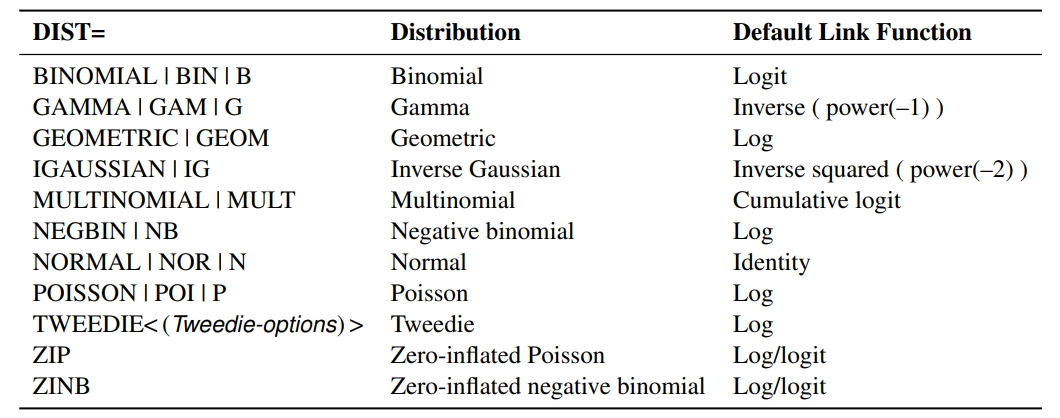
\includegraphics[width=1\textwidth]{link.jpg}
		\end{center}

	
	
\end{frame}
%------------------------------------------------------------------------------------------
%

\section{Poisson Regression}

%
%------------------------------- 슬라이드   --------------------------------------------------
\begin{frame}
	\frametitle{Count Data}
	
	\begin{itemize}
		\item Count data, in which there is no upper limit to the number of counts, usually fall into two types
				\bigskip
		\begin{itemize}
			\item Rates : counts per unit of time/area/distance, etc
			\item Contingency tables : counts cross-classified by categorical variables
		\end{itemize}
		\bigskip
		\item We concentrate on rates data can be modelled using Poisson GLMs with a log link
	\end{itemize}
	
	
 \end{frame}
%------------------------------------------------------------------------------------------
%
%
%------------------------------- 슬라이드   --------------------------------------------------
\begin{frame}
	\frametitle{Poisson Regression Models}
	
	\begin{itemize}
		\item Log-linear model for mean rate:
		\[ \log(\lambda_i ) = \beta_0 + \beta_1 x_{1i} + \ldots +\beta_p x_{pi}
		\]
		where $p$ is the number of predictors (or covariates) in the model
		\bigskip
		\item Random component:
		\[ Y_i|\mathbf{X}_i \sim Poisson(\lambda_i )
		\]
		\smallskip
		\item Here, $\lambda_i = E(Y_i|\mathbf{X}_i)=var(Y_i|\mathbf{X}_i)$
	\end{itemize}
	
	\end{frame}
%------------------------------------------------------------------------------------------
%
%
%------------------------------- 슬라이드   --------------------------------------------------
\begin{frame}
	\frametitle{Exponentiating Poisson Regression Model}
	
	\begin{itemize}
		\item Exponentiating gives us a model for the rate parameter, or expected counts:
		\[ \lambda_i  = e^{\beta_0 + \beta_1 x_{1i} + \ldots +\beta_p x_{pi}}
		\]
				\bigskip
		\item For Poisson random variables, expectation of $Y_i$ is $\lambda_i$, so the log-linear model provides a prediction for the expected value of $Y_i$
	\end{itemize}
	
	
\end{frame}
%------------------------------------------------------------------------------------------
%
%
%------------------------------- 슬라이드   --------------------------------------------------
\begin{frame}
	\frametitle{Interpretation of the parameters}
	
	\begin{itemize}
		\item $e^{\beta_j}$=Rate ratio for a $1$ unit increase in $x_j$, i.e. rate ratio for $x_j +1$ compared to $x_j$, with other covariates held constant.
		\bigskip
		\item $e^{\Delta\beta_j}$=Rate ratio for a $\Delta$ unit increase in $x_j$, i.e. rate ratio for $x_j +\Delta$ compared to $x_j$, with other covariates held constant.
		\bigskip
		\item $e^{\beta_0}$=Baseline rate value, i.e. rate for an observation with all $X$'s equal to zero.
	\end{itemize}
	
	
\end{frame}
%------------------------------------------------------------------------------------------
%
%
%------------------------------- 슬라이드   --------------------------------------------------
\begin{frame}
	\frametitle{Why Molel on the Log Scale?}
	
	\begin{itemize}
		\item The systematic portion of the model allows linear combinations of the covariates:
		\[ \beta_0 + \beta_1 x_{1i} + \ldots +\beta_p x_{pi}
		\]
		
		\item Since we have no restrictions on the predictors $X_1 , \ldots, X_p$, the predicted values can take any values on the real line: $(-\infty, +\infty)$
		\bigskip
		\item But our outcome variable $Y_i$ consistes of counts, so the expected value of $Y_i$ has the restriction: $\lambda_i \in \left[0, +\infty\right)$
		\bigskip
		\item After taking a log transform, we get: $\log(\lambda_i) \in (-\infty, +\infty)$ which is just what we wanted.
	\end{itemize}
	
	
\end{frame}
%------------------------------------------------------------------------------------------
%
%
%------------------------------- 슬라이드   --------------------------------------------------
\begin{frame}
	\frametitle{Example: Danish Lung Cancer Counts}
	
	\begin{itemize}
		\item Cases of lung cancer were counted in four Danish cities between $1968$ and $1971$ inclusive.
		\bigskip
		\item We have $24$ observations on each of $4$ variables:
		\begin{itemize}
			\item Cases: the number of lung cancer cases
			\item Pop: the popilation of each age group in each city
			\item Age: the categorical age group; one of 40-54, 55-59, 60-64, 65-69, 70-74 or $>$74
			\item city: the city; one of Fredericia, Horsens, Kolding, or Vejle
		\end{itemize}
		\bigskip
		\item Questions of interest: How does the expected number of lung cancer counts vary by age?
	\end{itemize}
	
	
\end{frame}
%------------------------------------------------------------------------------------------
%
%
%------------------------------- 슬라이드   --------------------------------------------------
\begin{frame}
	\frametitle{Example: Danish Lung Cancer Counts}
	
	\begin{itemize}
		\item Dataset
		\begin{center}
			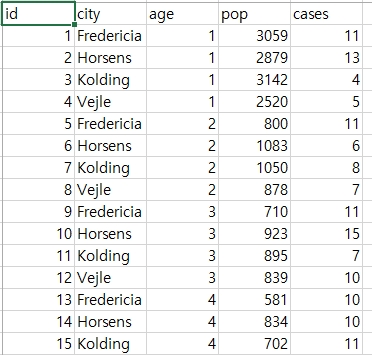
\includegraphics[width=0.6\textwidth]{dataset.jpg}
		\end{center}
	\end{itemize}
	
	
\end{frame}
%------------------------------------------------------------------------------------------
%
%
%------------------------------- 슬라이드   --------------------------------------------------
\begin{frame}
	\frametitle{Some Plots to Get Started}
	
	\begin{itemize}
		\item Boxplots of observed counts versus age category
		\begin{center}
			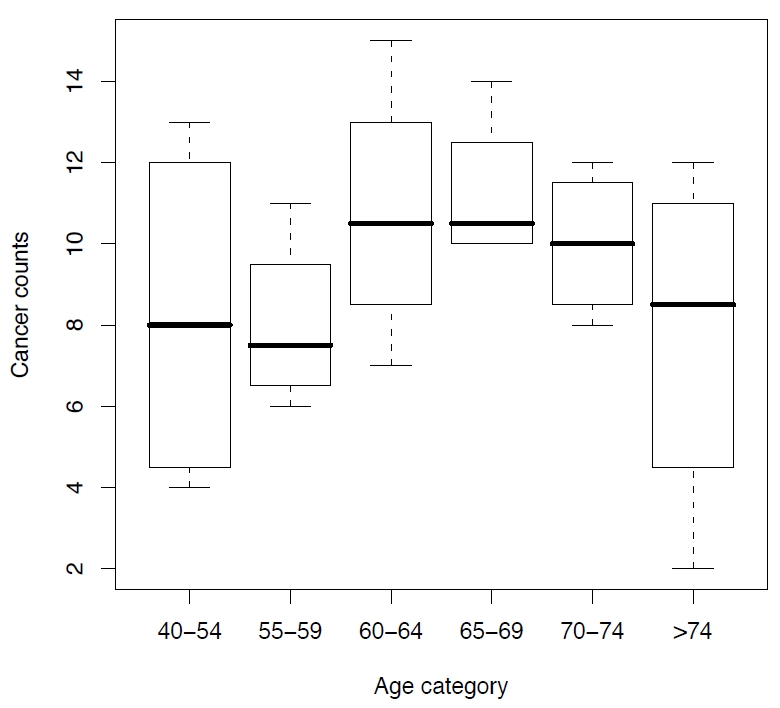
\includegraphics[width=0.6\textwidth]{boxplot.jpg}
		\end{center}
	\end{itemize}
	
	
\end{frame}
%------------------------------------------------------------------------------------------
%
%
%
%------------------------------- 슬라이드   --------------------------------------------------
\begin{frame}
	\frametitle{Model: Account for Age Only}
	
	\begin{itemize}
		\item Model
		\begin{eqnarray*}
			&&\log(\lambda_i )\\
			&=& \beta_0 +\beta_1 I(Age55-59_i)+\beta_2 I(Age60-64_i) \\
			&+&\beta_3 I(Age65-69_i)+\beta_4 I(Age70-74_i)+\beta_5 I(Age>74_i)
		\end{eqnarray*} 
		
		\item We are fitting a model with indicators for each of the age categories.
				\bigskip
		\item Baseline is the group aged $40-54$.
				\bigskip
		\item $I(age55-59)$ is an indicator of having age $55-59$, it is equal to $1$ for those of age $55-59$ and $0$ otherwise.
				\bigskip
		\item $I(age60-64)$ is an indicator of having age $60-64$, it is equal to $1$ for those of age $60-64$ and $0$ otherwise.
		\item etc...
	\end{itemize}
	
	
\end{frame}
%------------------------------------------------------------------------------------------
%
%
%------------------------------- 슬라이드   --------------------------------------------------
\begin{frame}
	\frametitle{Model: Account for Age Only}
	
	\begin{block}{SAS Code for Poisson regression}
		proc genmod data=danish; \\
		class age(ref='age40-54'); \\
		model cases=age/ \textbf{dist=poisson link=log} type3; \\
		estimate 'age2' age 1 0 0 0 0 -1/exp;\\
		estimate 'age3' age 0 1 0 0 0 -1/exp;\\
		estimate 'age4' age 0 0 1 0 0 -1/exp;\\
		estimate 'age5' age 0 0 0 1 0 -1/exp;\\
		estimate 'age6' age 0 0 0 0 1 -1/exp;\\
		run;
	\end{block}
	
	
\end{frame}
%------------------------------------------------------------------------------------------
%
%
%------------------------------- 슬라이드   --------------------------------------------------
\begin{frame}
	\frametitle{Model: Account for Age Only}
	
	\begin{itemize}
		\item Results
		\begin{center}
			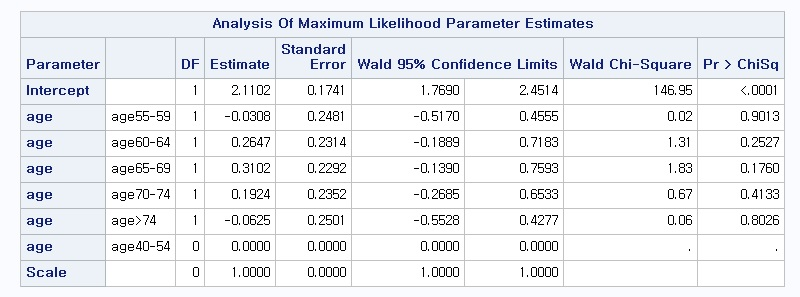
\includegraphics[width=0.9\textwidth]{result1.jpg}
		\end{center}
	\end{itemize}
	
	
\end{frame}
%------------------------------------------------------------------------------------------
%
%
%------------------------------- 슬라이드   --------------------------------------------------
\begin{frame}
	\frametitle{Model: Account for Age Only}
	
	\begin{itemize}
		\item[]	\begin{eqnarray*}
			\log(\lambda_i ) &=& 2.110 -0.031 I(Age55-59_i)+0.265 I(Age60-64_i) \\
			&+&0.310 I(Age65-69_i)+0.192 I(Age70-74_i)\\
			&-&0.063 I(Age>74_i)
		\end{eqnarray*} 
		
		\item We interpret $\hat{\beta}_0=2.110$ as the log expected count of cancer cases among individuals aged $40-54$
				\bigskip
		\item We interpret $\hat{\beta}_0+\hat{\beta}_1=2.079$ as the log expected count of cancer cases among individuals aged $55-59$
				\bigskip
		\item We interpret $\hat{\beta}_1=-0.031$ as the difference in log expected count of cancer cases comparing the $55-59$ age group to the $40-54$ age group. We can also interpret $\hat{\beta}_1$ as a log relative rate
	\end{itemize}
	
	
\end{frame}
%------------------------------------------------------------------------------------------
%

%
%------------------------------- 슬라이드   --------------------------------------------------
\begin{frame}
	\frametitle{Model: Account for Age Only}
	
	\begin{itemize}
		\item[]	\begin{eqnarray*}
			\log(\lambda_i ) &=& 2.110 -0.031 I(Age55-59_i)+0.265 I(Age60-64_i) \\
			&+&0.310 I(Age65-69_i)+0.192 I(Age70-74_i)\\
			&-&0.063 I(Age>74_i)
		\end{eqnarray*} 
		
		\item We interpret $exp(\hat{\beta}_0)=8.24$ as the expected count of cancer cases among individuals aged $40-54$
				\bigskip
		\item We interpret $exp(\hat{\beta}_0+\hat{\beta}_1)=8.00$ as the expected count of cancer cases among individuals aged $55-59$
				\bigskip
		\item We interpret $exp(\hat{\beta}_1)=0.97$ as the ratio of expected counts comparing the $55-59$ age group to the $40-54$ age group. We can also interpret $exp(\hat{\beta}_1)$ as a relative rate
	\end{itemize}
	
	
\end{frame}
%------------------------------------------------------------------------------------------
%

%
%------------------------------- 슬라이드   --------------------------------------------------
\begin{frame}
	\frametitle{Model: Account for Age Only}
	
	\begin{itemize}
		\item Let's perform a likelihood ratio test to look at the global hypothesis:
		\[ H_0 : \beta_1 = \beta_2 = \beta_3 = \beta_4 =\beta_5 =0
		\]
		versus the alternative hypothesis:
		\[ H_a : \text{at least one of the } \beta_i \text{'s is not } 0, \text{for } i\in 1,\ldots,5
		\] 
				\bigskip
		\item Test statistic:
		\item[] TS = -2(logLik(intercept only model)-logLik(Age model))
		\item[] \quad \hskip7pt    = 4.95 $\sim \chi_5^2$
				\bigskip
		\item Critical value for the hypothesis at level $\alpha=0.05$: $\chi_{5,0.05}^2 = 11.07$. Fail to reject the null hypothesis.
	\end{itemize}
	
	
\end{frame}
%------------------------------------------------------------------------------------------
%
%
%------------------------------- 슬라이드   --------------------------------------------------
\begin{frame}
	\frametitle{Model: Account for Age Only}
	
	\begin{itemize}
		\item[] Conclusions:
		\bigskip
		\item Based on the Poisson model of cancer case counts as a function of Age, we noted a generally increasing number of cases with increasing age.
		\bigskip
		\item The trend was not monotonically increasing with age.
		\bigskip
		\item Not a statistically significant result.
	\end{itemize}
	
	
\end{frame}
%------------------------------------------------------------------------------------------
%
%
%------------------------------- 슬라이드   --------------------------------------------------
\begin{frame}
	\frametitle{What About Accounting for Population Size?}
	
	\begin{itemize}
		\item So far we modelled the observed counts of cancer cases as Poisson counts.
				\bigskip
		\item The population size from each of these counts was drawn is also known.
				\bigskip
		\item Can we improve our analysis?
		\bigskip
		\item Each city and age group has a different population size.
				\bigskip
		\item If we model expected counts without accounting for population size, we may just be picking up effects of population distribution by age.
				\bigskip
		\item Accounting for population size can refine our analysis.
		
	\end{itemize}
	
	
\end{frame}
%------------------------------------------------------------------------------------------
%
%
%------------------------------- 슬라이드   --------------------------------------------------
\begin{frame}
	\frametitle{What About Accounting for Population Size?}
	
	\begin{itemize}
		\item The distribution of population sizes appears bimodal.
		\item The population sizes range from a minimum of $509$ to a miximum of $3,142$ people.
		\begin{center}
			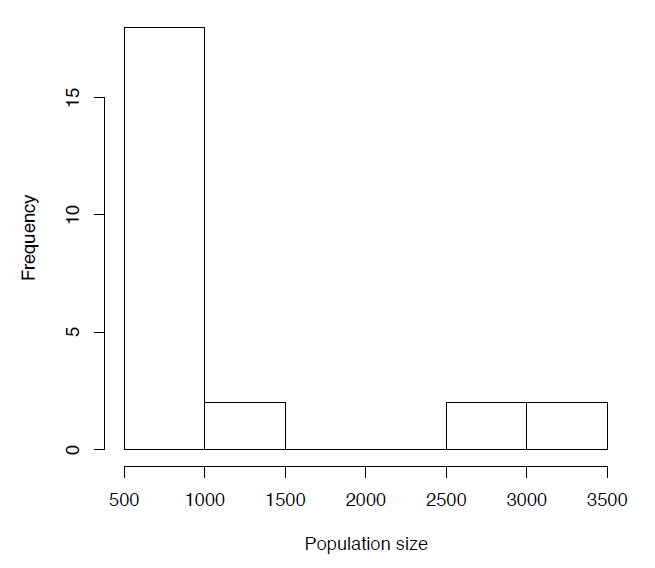
\includegraphics[width=0.6\textwidth]{dist.jpg}
		\end{center}
		
	\end{itemize}
	
	
\end{frame}
%------------------------------------------------------------------------------------------
%
%
%------------------------------- 슬라이드   --------------------------------------------------
\begin{frame}
	\frametitle{What About Accounting for Population Size?}
	
	\begin{itemize}
		\item So far, we have modeled expected counts for each population group, within the $4$ year period of time:
		\[ Rate=Counts/4years
		\]
		\item It may be more intersting to know the rate per person, per $4$ year period of time:
		\[ Rate=\frac{Counts/Population\ size}{4\ years} = \frac{Counts}{4\ person-years}
		\]
		\item Even better, we can get the rate per person year as:
		\[ Rate=\frac{Counts/4\ Population\ size}{4\ years} = \frac{Counts}{person-years}
		\]
	\end{itemize}
	
	
\end{frame}
%------------------------------------------------------------------------------------------
%

%------------------------------- 슬라이드   --------------------------------------------------
\begin{frame}
	\frametitle{What About Accounting for Population Size?}
	
	\begin{itemize}
		\item Here, $4\cdot Population\ size$ is equal to the number of person-years that we observed to obtain each count.
		\bigskip
		\item We can think of the person years at the denominator to be used to caculate the cancer rate per person, per year.
		\bigskip
		\item If we prefer the cancer rate per $100$ person-years, we can just multiply the rate per person-year by $100$.
	\end{itemize}
	
	
\end{frame}
%------------------------------------------------------------------------------------------
%

%------------------------------- 슬라이드   --------------------------------------------------
\begin{frame}
	\frametitle{Example: HIV infection rate}
	
	\begin{itemize}
		\item Suppose we are told that $100,000$ new cases of HIV were reported in the world, during the past three years.
		\item What is the incidence rate of HIV?
		\item We can calculate incidence as:
		\begin{eqnarray*}
			& &\frac{Number\ of\ new\ cases}{Number\ of\ people\ observed \cdot Amount\ of\ time\ observed} \\
			&=& \frac{100,000\ cases}{6,000,000,000\ people\ in\ the\ world \cdot 3\ years\ of\ observation}\\
			&=& 5.55 \times 10^{-6} \ cases / person - year \\
			&=& 5.55\ cases/ 1,000,000\ person - years
		\end{eqnarray*}
		Based on this incidence rate, we could say that each year, there are about $5.55$ new cases of HIV per $1,000,000$ people per year.
	\end{itemize}
	
	
\end{frame}
%------------------------------------------------------------------------------------------
%

%------------------------------- 슬라이드   --------------------------------------------------
\begin{frame}
	\frametitle{Model: Danish Cancer Cases with an Offset}
	
	\begin{itemize}
		\item So far, we have written a model for the expected number of counts over the $4$ year period of observation.
		\item However, if we know that the total populations generating our counts differ substantially, it does not make sense to write a log-linear model to consider expected counts direct.
		\item What we really wnat is to consider, the rate per person year
		\[ r_i = \frac{\lambda_i } {Pop_i}=\frac{E(count_i )}{Pop_i}
		\]
		and model that by a log-linear model.
		\item Based on this model, we can still say:
		\[ Y_i \sim Poisson(\lambda_i )=Poisson(r_i \cdot Pop_i)
		\]
	\end{itemize}
	
	
\end{frame}
%------------------------------------------------------------------------------------------
%

%------------------------------- 슬라이드   --------------------------------------------------
\begin{frame}
	\frametitle{Model: Danish Cancer Cases with an Offset}
	
	\begin{itemize}
		
		\item On a log scale, our model will be: 	
		\begin{eqnarray*}
			\log(r_{i})&=&\log(\frac{\lambda_i}{Pop_i} )=\beta_0 +\beta_1 I(Age55-59_i)+\beta_2 I(Age60-64_i) \\
			&+&\beta_3 I(Age65-69_i)+\beta_4 I(Age70-74_i)+\beta_5 I(Age>74_i)
		\end{eqnarray*} 
		
		\item Exponentiating, we get:
		\begin{eqnarray*}
			\frac{\lambda_i}{Pop_i} &=& exp\{ \beta_0 +\beta_1 I(Age55-59_i)+\beta_2 I(Age60-64_i) \\
			&+&\beta_3 I(Age65-69_i)+\beta_4 I(Age70-74_i)+\beta_5 I(Age>74_i) \}
		\end{eqnarray*} 
		\item Divide the $\lambda_i$s by the population size that yielded each count to get rates "per $4$ person-years".
	\end{itemize}
	
	
\end{frame}
%------------------------------------------------------------------------------------------
%

%------------------------------- 슬라이드   --------------------------------------------------
\begin{frame}
	\frametitle{Model: Danish Cancer Cases with an Offset}
	
	\begin{itemize}
		
		\item Now that we have a model of rates per $4$ person-years, we can divide by $4$ to get rate per person-year.
				\bigskip
		\item We can then multiply by $10,000$ to get rates per $10,000$ person-years (maybe easier to interpret than person-years).
				\bigskip
		\item Dividing by 4 and multiplying by $10,000$ is the same as multiplying by $2500$:
				\bigskip
		\item Exponentiating, we get:
		\begin{eqnarray*}
			&&\frac{\lambda_i}{Pop_i/2500} = exp\{ \beta_0 +\beta_1 I(Age55-59_i)+\beta_2 I(Age60-64_i) \\
			&+&\beta_3 I(Age65-69_i)+\beta_4 I(Age70-74_i)+\beta_5 I(Age>74_i) \}
		\end{eqnarray*} 
	\end{itemize}
	
	
\end{frame}
%------------------------------------------------------------------------------------------
%

%------------------------------- 슬라이드   --------------------------------------------------
\begin{frame}
	\frametitle{Model: Danish Cancer Cases with an Offset}
	
	\begin{itemize}
		
		\item Finally, we should take a log-transform to get back our log-linear model: 	
		\begin{eqnarray*}
			&&\log(\frac{\lambda_i}{Pop_i /2500} ) \\
			&=&\beta_0 +\beta_1 I(Age55-59_i)+\beta_2 I(Age60-64_i) \\
			&+&\beta_3 I(Age65-69_i)+\beta_4 I(Age70-74_i)+\beta_5 I(Age>74_i)
		\end{eqnarray*} 
		
		\item Further, we can move the population denominator to the other size of the equation:
		\begin{eqnarray*}
			&&\log(\lambda_i ) \\
			&=& \log(Pop_i/2500) + \beta_0 +\beta_1 I(Age55-59_i)+\beta_2 I(Age60-64_i) \\
			&+&\beta_3 I(Age65-69_i)+\beta_4 I(Age70-74_i)+\beta_5 I(Age>74_i) 
		\end{eqnarray*} 
	\end{itemize}
	
	
\end{frame}
%------------------------------------------------------------------------------------------
%

%------------------------------- 슬라이드   --------------------------------------------------
\begin{frame}
	\frametitle{Model: Danish Cancer Cases with an Offset}
	
	\begin{itemize}
		
		\item Here, we call the amount $\log(Pop_i/2500)$ the \textbf{offset}.
				\bigskip
		\item using the offset is just a way of accounting for population sizes, which could vary by age, region, etc.
				\bigskip
		\item The term "offset" is jargon for predictor terms whose $\beta$ coefficient is forced to be $+1$.
				\bigskip
		\item Using an offset gives us a convenient way to model rates per person-years, instead of just modeling the raw counts.
				\bigskip
		\item If all the observations have the same exposure, the model does not need an offset term and we can model $\log(\lambda_i)$ directly.
	\end{itemize}
	
	
\end{frame}
%------------------------------------------------------------------------------------------
%
%
%------------------------------- 슬라이드   --------------------------------------------------
\begin{frame}
	\frametitle{Model: Danish Cancer Cases with an Offset}
	
	\begin{block}{SAS Code for Poisson regression}
		data danish;\\
		set danish;\\
		logpop=log(pop/2500);\\
		run;\\
		
		proc genmod data=danish; \\
		class age(ref='age40-54'); \\
		model cases=age/\textbf{offset=logpop} dist=poisson link=log type3; \\
		estimate 'age2' age 1 0 0 0 0 -1/exp;\\
		estimate 'age3' age 0 1 0 0 0 -1/exp;\\
		estimate 'age4' age 0 0 1 0 0 -1/exp;\\
		estimate 'age5' age 0 0 0 1 0 -1/exp;\\
		estimate 'age6' age 0 0 0 0 1 -1/exp;\\
		run;
	\end{block}
	
	
\end{frame}
%------------------------------------------------------------------------------------------
%
%
%------------------------------- 슬라이드   --------------------------------------------------
\begin{frame}
	\frametitle{Model: Danish Cancer Cases with an Offset}
	
	\begin{itemize}
		\item Results
		\begin{center}
			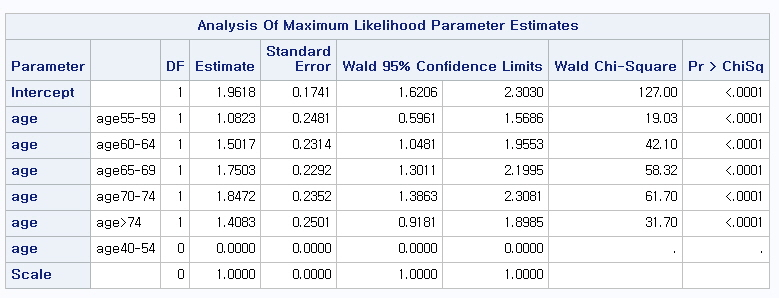
\includegraphics[width=0.9\textwidth]{result2.jpg}
		\end{center}
	\end{itemize}
	
	
\end{frame}
%------------------------------------------------------------------------------------------
%
%
%------------------------------- 슬라이드   --------------------------------------------------
\begin{frame}
	\frametitle{Model: Danish Cancer Cases with an Offset}
	
	\begin{itemize}
		\item After including the offset in our model, we need to change our regression coefficient interpretations a bit.
				\bigskip
		\item We should think of the outcome as $\log(\lambda_i)-\text{offset}_i$.
				\bigskip
		\item In this case, $\lambda_i$ was the expected number of cases observed in a particular age group and city, within a $4$ year period of time.
		\bigskip
		\item Our offset was $\log(Pop_i/2500)$.
				\bigskip
		\item So, we should think of the outcome as log rate per $10,000$ person years.
	\end{itemize}
	
	
\end{frame}
%------------------------------------------------------------------------------------------
%
%
%------------------------------- 슬라이드   --------------------------------------------------
\begin{frame}
	\frametitle{Model: Danish Cancer Cases with an Offset}
	
	\begin{itemize}
		\item $\beta_0$ is the log rate of cancer cases per $10,000$ person years in the baseline age group of $40-54$.
		\bigskip
		\item $\beta_1$ is the log relative rate of cancer cases per $10,000$ person years comparing the age group $55-59$ to the baseline age group $40-54$.
		\bigskip
		\item $\beta_2$ is the log relative rate of cancer cases per $10,000$ person years comparing the age group $60-64$ to the baseline age group $40-54$.
	\end{itemize}
	
	
\end{frame}
%------------------------------------------------------------------------------------------
%
%
%------------------------------- 슬라이드   --------------------------------------------------
\begin{frame}
	\frametitle{Model: Danish Cancer Cases with an Offset}
	
	\begin{itemize}
		\item Before we put the offset in our model, none of our regression coefficients were statistically significant.
		\smallskip
		\item[] $\Rightarrow$ without the offset, there was no statistically sifnificant difference in the expected counts per year at age group compared to the baseline $40-54$ group.
		\bigskip
		\item After including the offset, we're looking for differences in the expected counts per person-year, across age groups. 
	\end{itemize}
	
	
\end{frame}
%------------------------------------------------------------------------------------------
%
%
%------------------------------- 슬라이드   --------------------------------------------------
\begin{frame}
	\frametitle{Model: Danish Cancer Cases with an Offset}
	
	\begin{itemize}
		\item Let's perform a likelihood ratio test to look at the global hypothesis:
		\[ H_0 : \beta_1 = \beta_2 = \beta_3 = \beta_4 =\beta_5 =0
		\]
		versus the alternative hypothesis:
		\[ H_a : \text{at least one of the } \beta_i \text{'s is not } 0, \text{for } i\in 1,\ldots,5
		\] 
				\bigskip
		\item Test statistic:
		\item[] TS = -2(logLik(intercept only, with offset)-logLik(Age model with offset)) = 101.6 $\sim \chi_5^2$
				\bigskip
		\item Critical value for the hypothesis at level $\alpha=0.05$: $\chi_{5,0.05}^2 = 11.07$. reject the null hypothesis.
	\end{itemize}
	
	
\end{frame}
%------------------------------------------------------------------------------------------
%
%------------------------------- 슬라이드   --------------------------------------------------
\begin{frame}
	\frametitle{Model: Danish Cancer Cases with an Offset}
	
	\begin{itemize}
		\item Model
		\begin{eqnarray*}
			&&\log(\lambda_i ) \\
			&=& \log(Pop_i/2500) + \beta_0 +\beta_1 I(Age55-59_i)+\beta_2 I(Age60-64_i) \\
			&+&\beta_3 I(Age65-69_i)+\beta_4 I(Age70-74_i)+\beta_5 I(Age>74_i) 
		\end{eqnarray*} 
		\item Predicted log rate of cancer per $10,000$ person years among $40-54$ year olds;
		\[ \hat{\beta}_0=1.96
		\]
		\item Predicted rate of cancer per $10,000$ person years among $40-54$ year olds;
		\[ exp(\hat{\beta}_0)=exp(1.96)=7.09
		\]
		\item Based on this model, we predict $7.09$ new cases of lung cancer per $10,000$ $40-54$ year olds in Denmark, per year.
	\end{itemize}
	
	
\end{frame}
%------------------------------------------------------------------------------------------
%
%
%------------------------------- 슬라이드   --------------------------------------------------
\begin{frame}
	\frametitle{Model: Danish Cancer Cases with an Offset}
	
	\begin{itemize}
		\item Predicted log rate of cancer per $10,000$ person years among $55-59$ year olds;
		\[ \hat{\beta}_0 + \hat{\beta}_1=3.04
		\]
		\item Predicted rate of cancer per $10,000$ person years among $55-59$ year olds;
		\[ exp(\hat{\beta}_0 + \hat{\beta}_1)=exp(1.96+1.08)=20.9
		\]
				\bigskip
		\item Based on this model, we predict $20.9$ new cases of lung cancer per $10,000$ $55-59$ year olds in Denmark, per year.
	\end{itemize}
	
	
\end{frame}
%------------------------------------------------------------------------------------------
%
%
%------------------------------- 슬라이드   --------------------------------------------------
\begin{frame}
	\frametitle{Model: Danish Cancer Cases with an Offset}
	
	\begin{itemize}
		\item We predicted an incidence rate of $7.09$ cases per $10,000$ per year among $40-54$ year olds, and a rate of $20.9$ new cases per $10,000$ person years for $55-59$ years olds.
		\bigskip
		\item[] $\Rightarrow$ The relative rate per $10,000$ person years comparing $55-59$ years olds to $40-54$ years olds is $20.9/7.09 \approx 2.94$.
			\bigskip
		\item We could have gotten the same answer by taking $exp(\hat{\beta}_1)=exp(1.08)=2.94$.
			\bigskip
		\item $exp(\hat{\beta}_1)$ is the relative rate cancer cases per $10,000$ person years comparing $55-59$ years olds to $40-54$ years olds.
			\bigskip
		\item $\hat{\beta}_1$ is the log relative rate.  
	\end{itemize}
	
	
\end{frame}
%------------------------------------------------------------------------------------------
%
%
%------------------------------- 슬라이드   --------------------------------------------------
\begin{frame}
	\frametitle{Model: Danish Cancer Cases with an Offset}
	
	\begin{itemize}
		\item There is an increasing trend in relative rates compared to the baseline $40-54$ year old group as age increases.
		\bigskip
		\item The only exception for this trend is for the $Age>74$ group.
		\bigskip
		\item The model fit matches what we know from biology: the risk of cancer does increase with age, but trails of for the oldest individuals perhaps because
		\begin{itemize}
			\item Those surviving to age $74$ and beyond have genes which protect against cancer.
			\item Cell growth slows down at older ages, slowing the growth of tumors.
		\end{itemize}
	\end{itemize}
	
	
\end{frame}
%------------------------------------------------------------------------------------------
%
%
%------------------------------- 슬라이드   --------------------------------------------------
\begin{frame}
	\frametitle{Some Additional Notes about Offsets}
	
	\begin{itemize}
		\item The purpose of an offset is the change the denominator or units of a rate.
		\bigskip
		\item Often, the model without an offset does not make much sense, and likely fails our Poisson assumptions.
			\bigskip
		\item We should always try to use an offset if we suspect that the underlying population sizes differ for each of the observed counts.
			\bigskip
		\item Typically the offset will take value $\log(N)$ where $N$ is the sample size, or the number of person-years.
			\bigskip
		\item If the underlying population sizes are not available, we just have to do our best - but be careful about applying the Poisson model.
	\end{itemize}
	
	
\end{frame}
%------------------------------------------------------------------------------------------
%

%
%------------------------------- 슬라이드   --------------------------------------------------
\begin{frame}
	\frametitle{Summary}
	
	\begin{itemize}
		\item Log-linear models can be a good way to approach count data.
		\bigskip
		\item If population sizes or denominators are available, it's a good idea to include an offset.
		\bigskip
		\item Log-linear models can also be useful in analyzing binary data from cohort studies, but with care.
	\end{itemize}
	
	
\end{frame}
%------------------------------------------------------------------------------------------
%
\section{Logistic regression}

%
%------------------------------- 슬라이드   --------------------------------------------------
\begin{frame}
	\frametitle{Logistic Regression Models}
	
	\begin{itemize}
		\item 로지스틱 회귀분석은 특정 질병의 유무에 영향을 미치는 요인을 밝히는 통계적 방법
		\bigskip
		\item 종속변수가 범주형 자료인 경우 연속형 자료를 종속변수로 이용하는 회귀분석은 사용 불가능. 이때 로지스틱 회귀분석을 이용
		\bigskip
		\item 선형회귀모형
		\[ 	y = \beta_0 + \beta_1 x_{1} + \ldots + \beta_p x_{p} + \epsilon
		\]
		\smallskip
		\item 로지스틱 회귀모형
			\[ \log(\frac{p}{1-p})= \beta_0 + \beta_1 x_{1} + \ldots + \beta_p x_{p} 
			\]
		\item[] 여기서 $p$는 성공(예: 질환의 발병) 확률을 의미
	\end{itemize}
	
	
\end{frame}
%------------------------------------------------------------------------------------------
%
%
%------------------------------- 슬라이드   --------------------------------------------------
\begin{frame}
	\frametitle{Logistic Regression Models}
	
	\begin{itemize}
		\item 체중($X$)과 고혈압 유무($P$) 관계 그래프
			\begin{center}
				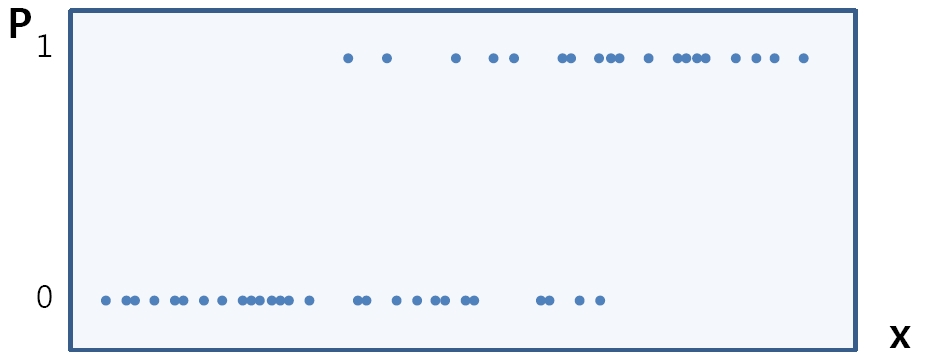
\includegraphics[width=0.8\textwidth]{lo1.jpg}
			\end{center}
			\bigskip
		\item 체중이 증가함에 따라 고혈압이 있을 확률이 증가
		\bigskip
		\item 고혈압 여부는 연속형 변수가 아닌 $0$과 $1$의 두 가지 값을 갖는 이분형 변수이기 때문에 선형회귀 분석 불가
	\end{itemize}
	
	
\end{frame}
%------------------------------------------------------------------------------------------
%
%
%------------------------------- 슬라이드   --------------------------------------------------
\begin{frame}
	\frametitle{Logistic Regression Models}
	
	\begin{itemize}
		\item 위험요인(체중)의 각 수준에 따른 질병(고혈압)이 있을 확률 $p$를 로짓변환(logit transformation)해 주면 $logit(p)$는 $-\infty \sim \infty$의 연속형 변수로 변환됨
		\bigskip 
		\item 로짓변환
		\[ logit(p)=\ln \frac{p}{1-p}
		\]
		\begin{center}
			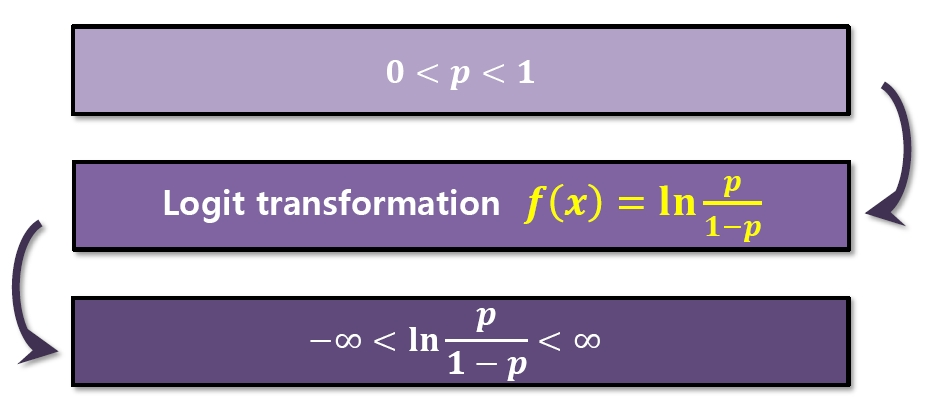
\includegraphics[width=0.8\textwidth]{lo2.jpg}
		\end{center}
		\bigskip
		\item 로지스틱 회귀분석은 $logit(p)$를 종속변수로 두고 회귀분석을 적용한 방법
		
	\end{itemize}
	
	
\end{frame}
%------------------------------------------------------------------------------------------
%
%
%------------------------------- 슬라이드   --------------------------------------------------
\begin{frame}
	\frametitle{Logistic Regression Models}
	
	\begin{itemize}
		\item 질병이 있을 확률 $p$ 추정
		\begin{center}
			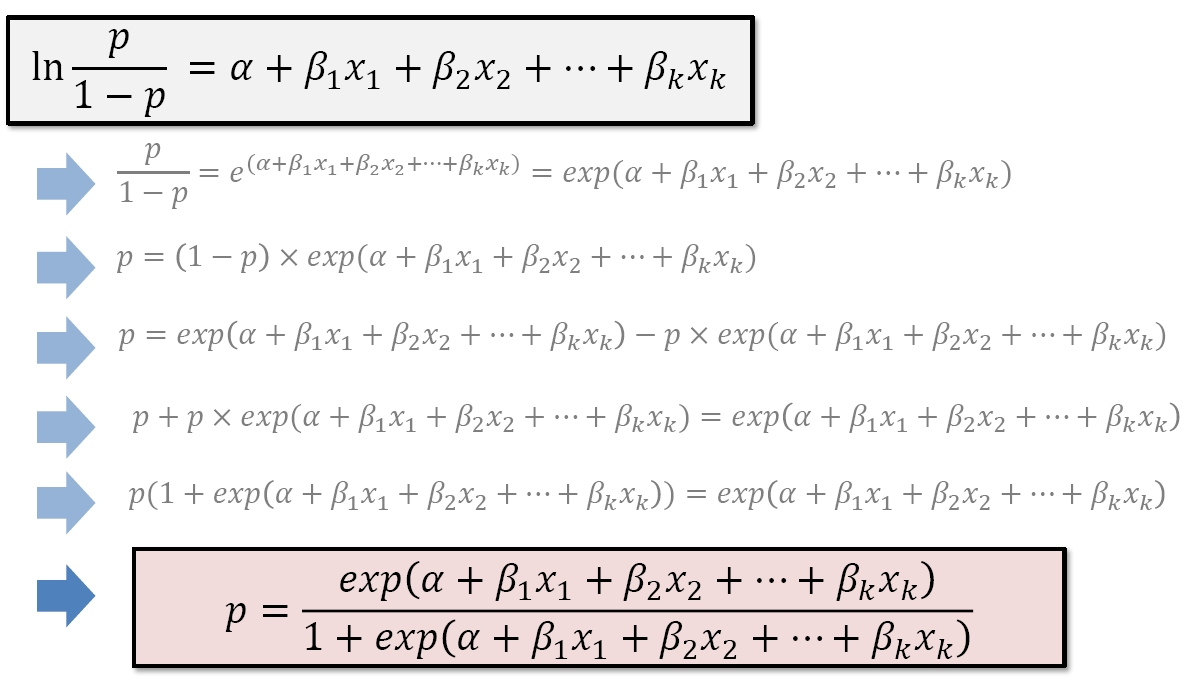
\includegraphics[width=0.8\textwidth]{lo3.jpg}
		\end{center}


		
	\end{itemize}
	
	
\end{frame}
%------------------------------------------------------------------------------------------
%

%
%------------------------------- 슬라이드   --------------------------------------------------
\begin{frame}
	\frametitle{Logistic Regression Models}
	
	\begin{itemize}
		\item 확률 곡선
		\begin{center}
			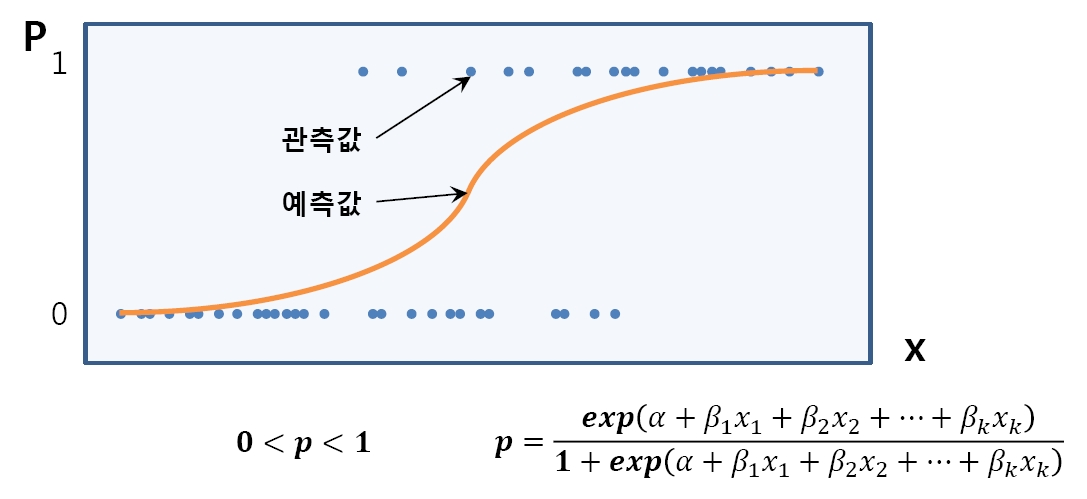
\includegraphics[width=0.6\textwidth]{lo4.jpg}
		\end{center}
	\item 로지스틱 회귀 직선
				\begin{center}
					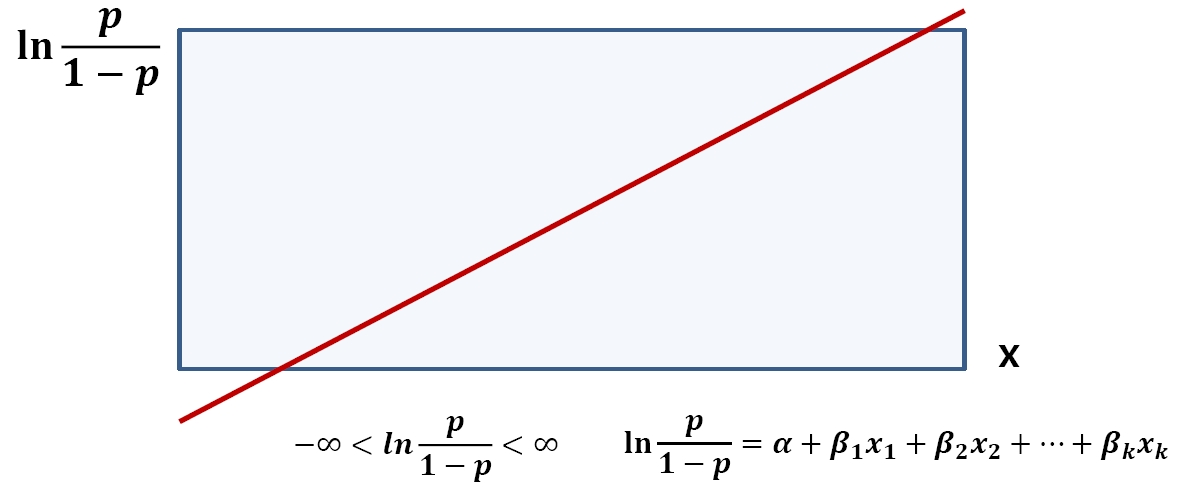
\includegraphics[width=0.6\textwidth]{lo5.jpg}
				\end{center}
		
	\end{itemize}
	
	
\end{frame}
%------------------------------------------------------------------------------------------
%

%
%------------------------------- 슬라이드   --------------------------------------------------
\begin{frame}
	\frametitle{Logistic Regression Models}
	
	\begin{itemize}
		\item 로지스틱 회귀분석은 질병이 있을 확률을 기준으로 질병 여부에 대한 예측 가능
		\bigskip
		\item 예측의 정확도는 분류표를 통해 산출 가능
		\bigskip
		\item 분류표
		\begin{center}
			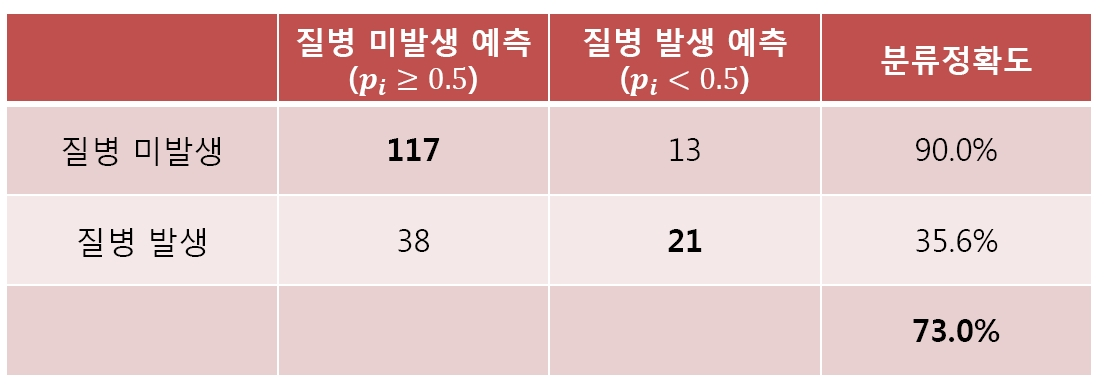
\includegraphics[width=0.9\textwidth]{lo6.jpg}
		\end{center}
		
	\end{itemize}

	
\end{frame}
%------------------------------------------------------------------------------------------
%
%
%------------------------------- 슬라이드   --------------------------------------------------
\begin{frame}
	\frametitle{Logistic Regression Models}
	
	\begin{itemize}
		\item 회귀 계수의 해석
				\begin{center}
					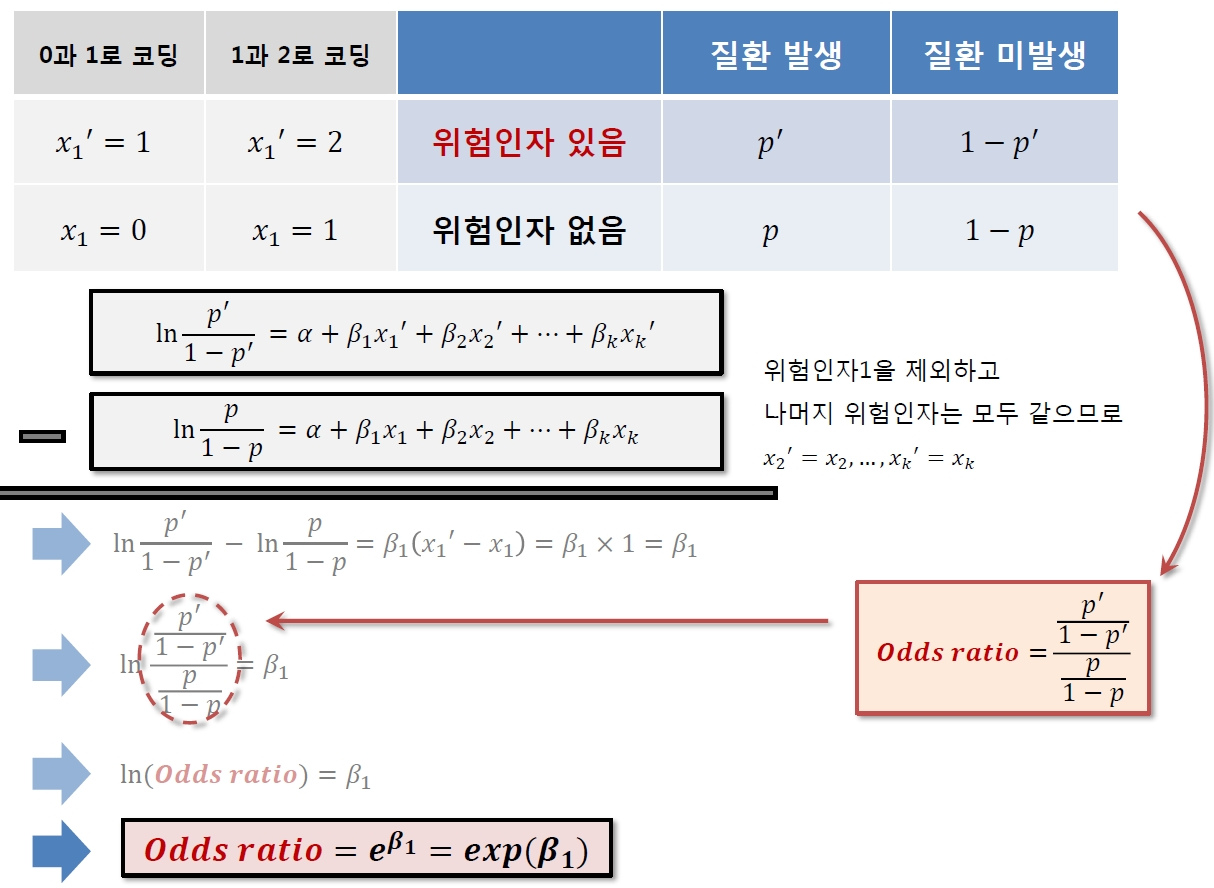
\includegraphics[width=0.8\textwidth]{lo7.jpg}
				\end{center}
	\end{itemize}
	
	
\end{frame}
%------------------------------------------------------------------------------------------
%
%
%------------------------------- 슬라이드   --------------------------------------------------
\begin{frame}
	\frametitle{Logistic Regression Models}
	
	\begin{itemize}
		\item 로지스틱 회귀분석에서 개별 위험인자의 영향은 $exp(\beta)$값을 통해 질병 발생에 대한 교차비(odds ratio)로 표현
\bigskip
\item 교차비가 1인 경우 요인과 질병은 전혀 관계가 없으며, 1보다 크면 요인에 의해 질병의 위험이 증가, 1보다 작으면 감소함을 의미
\bigskip
\item 위험인자와 질병의 관련성을 표현할때는 교차비, 유의수준, 교차비의 $95\%$ 신뢰구간을 동시에 제시하는 것이 좋음
\bigskip
\item 교차비의 $95\%$ 신뢰구간과 $p$-value
				\begin{center}
					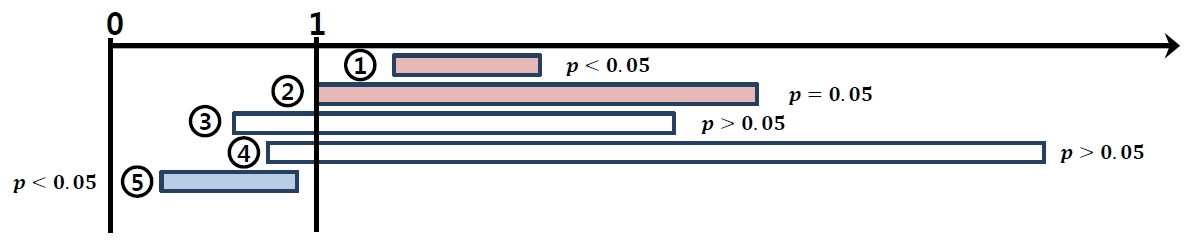
\includegraphics[width=0.9\textwidth]{lo8.jpg}
				\end{center}
	\end{itemize}
	
	
\end{frame}
%------------------------------------------------------------------------------------------
%
%
%------------------------------- 슬라이드   --------------------------------------------------
\begin{frame}
	\frametitle{Logistic Regression Models}
	
	\begin{itemize}
		\item 모형 적합도를 평가하는 방법으로 Hosmer-Lemeshow의 적합도 검정(goodness-of-fit test)을 이용
		\bigskip
		\item 가설
		\item[] $H_0$ : 로짓에 대한 회귀모형이 적합하다.
		\item[] $H_1$ : 모형이 적합하지 않다.
		\bigskip
		\item Hosmer-Lemeshow 검정은 표본크기가 충분히 큰 경우에 적용
		\bigskip 
		\item 일반적으로 모형계수 전체 검정(model chi-square test)을 이용하여 모형 적합도를 검정
		\bigskip
				\item 가설
				\item[] $H_0$ : 모든 $\beta_i =0$이다.
				\item[] $H_1$ : 최소한 하나의 $\beta_i$는 $0$이 아니다.
	\end{itemize}
	
	
\end{frame}
%------------------------------------------------------------------------------------------
%
%
%------------------------------- 슬라이드   --------------------------------------------------
\begin{frame}
	\frametitle{Logistic Regression Models}
	
	\begin{itemize}
		\item 이 외에 분류 정확도를 이용해 모형을 판단
		\item Cox \& Snell의 결정계수($R_{cs}^2$)와 Nagelkerke의 결정계수($R_N^2$)를 통해 모형의 설명력 제시 
						\begin{center}
							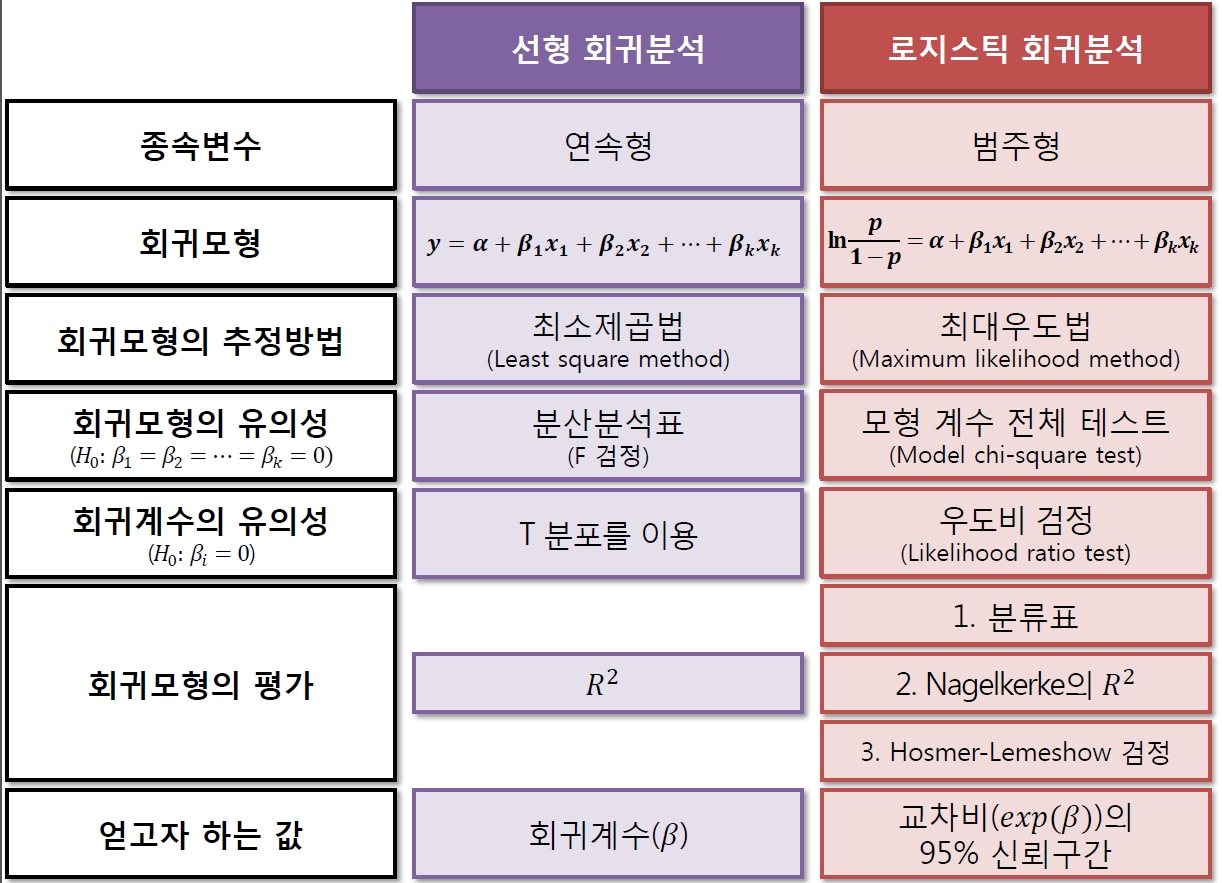
\includegraphics[width=0.7\textwidth]{lo9.jpg}
						\end{center}
	\end{itemize}
	
	
\end{frame}
%------------------------------------------------------------------------------------------
%

%------------------------------- 슬라이드  --------------------------------------------------
\begin{frame}
	\frametitle{Logistic Regression Models}
	
	\begin{example}
		다음은 1986년 미국의 Baystate Medical Center, Springfield에서 $189$명의 신생아 출산에 대한 자료이다. 출생 체중 $2.5kg$ 미만을 저체중 출산으로 정의한다. 이 자료를 통해 저체중 출산의 위험요인을 분석하라. 변수명은 차례로 저체중 여부, 산모 나이, 산모 체중, 인종, 흡연력, 조산 여부, 고혈압 유무, 자궁의 불안정성 여부이다.
		\begin{center}
			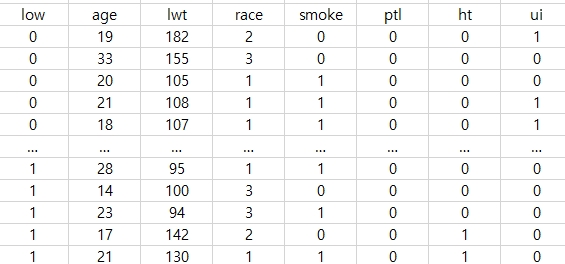
\includegraphics[width=0.8\textwidth]{ex1.jpg}
		\end{center}
	\end{example}
	
\end{frame}
%----------------------------------------------------------------------------------------------
%%


%
%------------------------------- 슬라이드  --------------------------------------------------
\begin{frame}
	\frametitle{Logistic Regression Models}
	
	\begin{block}{SAS Code}
		\begin{center}
			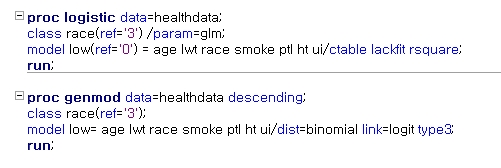
\includegraphics[width=1\textwidth]{ex2.jpg}
		\end{center} 
	\end{block}
	
\end{frame}
%----------------------------------------------------------------------------------------------
%%

%
%------------------------------- 슬라이드  --------------------------------------------------
\begin{frame}
	\frametitle{Logistic Regression Models}
	
	\begin{block}{Results}
		\begin{center}
			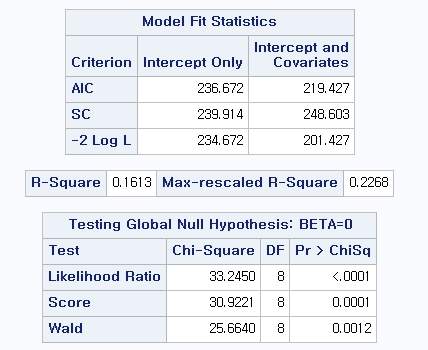
\includegraphics[width=0.6\textwidth]{ex3.jpg}
		\end{center} 
	\end{block}
	
\end{frame}
%----------------------------------------------------------------------------------------------
%%
%
%
%------------------------------- 슬라이드  --------------------------------------------------
\begin{frame}
	\frametitle{Logistic Regression Models}
	
	\begin{block}{Results}
		\begin{center}
			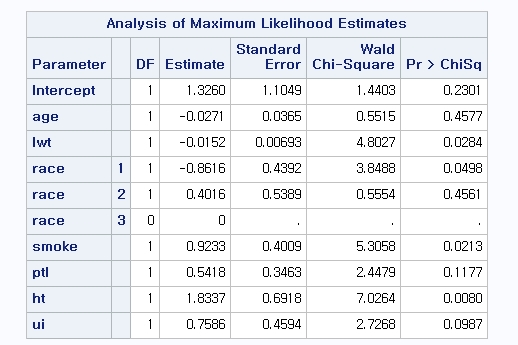
\includegraphics[width=0.8\textwidth]{ex4.jpg}
		\end{center} 
	\end{block}
	
\end{frame}
%----------------------------------------------------------------------------------------------
%%
%
%
%------------------------------- 슬라이드  --------------------------------------------------
\begin{frame}
	\frametitle{Logistic Regression Models}
	
	\begin{block}{Results}
		\begin{center}
			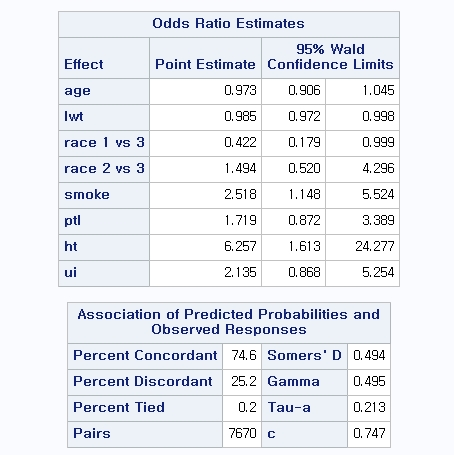
\includegraphics[width=0.5\textwidth]{ex5.jpg}
		\end{center} 
	\end{block}
	
\end{frame}
%----------------------------------------------------------------------------------------------
%%
%
%
%------------------------------- 슬라이드  --------------------------------------------------
\begin{frame}
	\frametitle{Logistic Regression Models}
	
	\begin{block}{Results}
		\begin{center}
			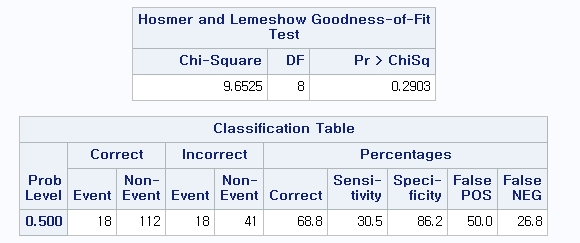
\includegraphics[width=0.9\textwidth]{ex6.jpg}
		\end{center} 
	\end{block}
	
\end{frame}
%----------------------------------------------------------------------------------------------
%%
%











%
%------------------------------- 슬라이드  --------------------------------------------------
\begin{frame}
	\begin{center}
		\includegraphics[width=0.6\textwidth]{thank.jpg}
	\end{center}
\end{frame}
%----------------------------------------------------------------------------------------------
%
\end{document}
%==========================  본문 끝 = ================================ 